% Homework template for Inference and Information
% UPDATE: September 26, 2017 by Xiangxiang
\documentclass[a4paper]{article}
\usepackage{amsmath, amssymb, amsthm}
% amsmath: equation*, amssymb: mathbb, amsthm: proof
\usepackage{moreenum}
\usepackage{mathtools}
\usepackage{url}
\usepackage{enumitem}
\usepackage{graphicx}
\usepackage{subcaption}
\usepackage{booktabs} % toprule
\usepackage[mathcal]{eucal}
\usepackage{xcolor}
\definecolor{dkgreen}{rgb}{0,0.6,0}
\definecolor{gray}{rgb}{0.5,0.5,0.5}
\definecolor{mauve}{rgb}{0.58,0,0.82}
\usepackage{listings}
\lstset{
  frame=tb,
  aboveskip=3mm,
  belowskip=3mm,
  showstringspaces=false,
  columns=flexible,
  framerule=1pt,
  rulecolor=\color{gray!35},
  backgroundcolor=\color{gray!5},
  basicstyle={\small\ttfamily},
  numbers=left,
  numberstyle=\tiny\color{gray},
  keywordstyle=\color{blue},
  commentstyle=\color{dkgreen},
  stringstyle=\color{mauve},
  breaklines=true,
  breakatwhitespace=true,
  tabsize=3,
  title=\lstname
}
%% Definitions for Inference and Information
%% UPDATE: September 26, 2017 by Xiangxiang 
\newcommand{\theterm}{Fall 2017}
\usepackage{xeCJK}
\usepackage{bm}

\newcommand{\thecoursename}{
Tsinghua University\\
%\vspace*{0.1in}
机器学习基础
}
\newcommand{\studentID}{2017310711}
\newcommand{\courseheader}{
\vspace*{-1in}
\begin{center}
\thecoursename \\
\theterm
\vspace*{0.1in}
\hrule
\end{center}
}
\newcommand{\NP}{$\mathcal{NP}$}
\newcommand{\rvx}{\mathsf{x}}    % x, r.v.
\newcommand{\rvy}{\mathsf{y}}    % y, r.v.
\newcommand{\rvz}{\mathsf{z}}    % z, r.v.
\newcommand{\urvx}{\underline{\mathsf{x}}}    % x, r.v. vec
\newcommand{\urvy}{\underline{\mathsf{y}}}    % y, r.v. vec
\newcommand{\urvz}{\underline{\mathsf{z}}}    % z, r.v. vec
\newcommand{\defas}{\triangleq} %\coloneqq
\newcommand{\reals}{\mathbb{R}}
%\newcommand{\T}{\mathrm{T}}    % transpose

% \newcommand{\E}[1]{\mathbb{E}\left[{#1}\right]}
% \newcommand{\Prob}[1]{\mathbb{P}\left({#1}\right)}
\DeclareMathOperator*{\argmax}{arg\,max}
\DeclareMathOperator*{\argmin}{arg\,min}
\DeclareMathOperator*{\argsup}{arg\,sup}
\DeclareMathOperator*{\arginf}{arg\,inf}
\DeclareMathOperator{\Var}{Var}
\DeclareMathOperator{\Cov}{Cov}
\DeclareMathOperator{\MSE}{MSE}
\DeclareMathOperator{\In}{\mathbb{I}}
\DeclareMathOperator{\E}{\mathbb{E}}
\DeclareMathOperator{\Prob}{\mathbb{P}}
\DeclareMathOperator{\sgn}{sgn}
\DeclareMathOperator\err{err}
\DeclareMathOperator\conv{conv}
\newcommand\independent{\protect\mathpalette{\protect\independenT}{\perp}}
\def\independenT#1#2{\mathrel{\rlap{$#1#2$}\mkern2mu{#1#2}}}
\usepackage{algorithmic}
\usepackage{algorithm}

\begin{document}
\courseheader

\newcounter{hwcnt}
\setcounter{hwcnt}{4} % set to the times of Homework

\begin{center}
  \underline{第\thehwcnt 次作业} \\
\end{center}
\begin{flushleft}
  赵丰\quad \studentID\hfill
  \today
\end{flushleft}
\hrule

\vspace{2em}

\flushleft
\rule{\textwidth}{1pt}
\begin{itemize}
\item {\bf Acknowledgments: \/} 
  This coursework refers to textbook.  
\item {\bf Collaborators: \/}
  \begin{itemize}
  \item DIY
  \end{itemize}
\end{itemize}
\rule{\textwidth}{1pt}

\vspace{2em}

I use \texttt{enumerate} to generate answers for each question:

\begin{enumerate}[label=\arabic*.]
  \setlength{\itemsep}{3\parskip}
  \item 
     \begin{enumerate}[label*=\arabic*.]
     \item 
    \begin{algorithm}
    \caption{modifed ADABOOST$(S=((x_1,y_1),\dots,(x_m,y_m)))$}\label{alg}
    \begin{algorithmic}[1]
    \FOR{$i=1$ to $m$}
    \STATE $D_1(i)\leftarrow \frac{1}{m}$
    \ENDFOR
    \FOR{$t=1$ to $T$}
    \STATE $h_t \leftarrow$ base classifier in $H$ with small error $\epsilon_t=\Pr_{i\sim D_t}[h_t(x_i)\neq y_i]$
    \STATE $Z_t \leftarrow (1-\epsilon_t)e^{-\alpha}+\epsilon_t e^{\alpha}$    
    \FOR{$i=1$ to $m$}
    \STATE $D_{t+1}(i)\leftarrow \frac{D_t(i)exp(-\alpha y_i h_t(x_i))}{Z_t}$    
    \ENDFOR        
    \ENDFOR    
    \STATE $g\leftarrow \sum_{t=1}^T h_t$
    \RETURN $h=\sgn(g)$        
    \end{algorithmic}
    \end{algorithm}

         设常数$\alpha=\frac{1}{2}\log\frac{1+2\gamma}{1-2\gamma}$,原adaboost算法按上表修改:
            相应的证明过程中首先有:
            \begin{align}
            D_{t+1}(i)=\frac{e^{-y_i g_t(i)\alpha}}{m\prod_{s=1}^t Z_s}
            \end{align}
            其中$g_t=\sum_{s=1}^t h_s$
            注意到算法中$Z_t$的取值是使得$\sum_{i=1}^m D_{t+1}(i)=1$,
            所以利用$1_{u\leq 0}\leq exp(-u\alpha)$得训练误差
            \begin{equation}
            \hat{R}(h)\leq \prod_{t=1}^T Z_t
            \end{equation}
         注意到$Z_t$是关于$\epsilon_t$的增函数,根据题目中$\epsilon_t\leq \frac{1}{2}-\gamma$得到
            \begin{align}
                Z_t\leq &(\frac{1}{2}+\gamma)e^{-\alpha}+(\frac{1}{2}-\gamma)e^{\alpha}\\
                = & \sqrt{1-4\gamma^2}
            \end{align}
            所以有
            \begin{equation}
            \hat{R}(h)\leq (1-4\gamma^2)^{\frac{T}{2}}
            \end{equation}            
        \item
        \begin{enumerate}[label=(\alph*)]
            \item 设已经有$\bm{\alpha}_{t-1}=(\alpha_1,\dots,\alpha_{t-1},0,\dots,0)$
            \begin{equation}
            \end{equation}            
            设$\epsilon_t$
            \begin{equation}
            \frac{d L(\bm{\alpha_{t-1}}+\eta \bm{e}_t)}{d\eta}|_{\eta=0}=\sum_{i=1}^m \Phi'(-y_i \sum_{j=1}^{t-1} \alpha_j h_j(x_i))(-y_i h_t(x_i))
            \end{equation}
            记
            \begin{equation}
            D_t(i)=\frac{\Phi'(-y_i \sum_{j=1}^{t-1}\alpha_j h_j(x_i))}{\sum_{i=1}^m\Phi'(-y_i \sum_{j=1}^{t-1}\alpha_j h_j(x_i))}
            \end{equation}            
            满足$\sum_{i=1}^m D_t(i)=1$。
            
            于是有:
            \begin{equation}
            \frac{d L(\bm{\alpha_{t-1}}+\eta \bm{e}_t)}{d\eta}|_{\eta=0}=-\sum_{i=1}^m D_t(i)y_i h_t(x_i)[\sum_{i=1}^m\Phi'(-y_i \sum_{j=1}^{s-1}\alpha_j h_j(x_i))]
            \end{equation}            
            假设$h_s(s\leq t-1)$已经取好,设$\epsilon_t=\Pr_{i\sim D_t}[h_t(x_i)\neq y_i]$
            则将上式可化为
            \begin{equation}
            \frac{d L(\bm{\alpha_{t-1}}+\eta \bm{e}_t)}{d\eta}|_{\eta=0}=-(2\epsilon_t-1)[\sum_{i=1}^m\Phi'(-y_i \sum_{j=1}^{s-1}\alpha_j h_j(x_i))]
            \end{equation}            
            为使$L$在$\bm{\alpha_{t-1}}$处的方向导数最小,取
            \begin{equation}
            h_t=\argmin_{h\in H} \Pr_{i\sim D_t}[h_t(x_i)\neq y_i]
            \end{equation}  
            为确定步长$\eta$,需求解$\frac{d L(\bm{\alpha_{t-1}}+\eta \bm{e}_t)}{d\eta}=0$,
            原Adaboost算法修改如表\ref{alg2}所示。
            \begin{algorithm}
            \caption{一般代价函数Adaboost$(S=((x_1,y_1),\dots,(x_m,y_m)))$}\label{alg2}
            \begin{algorithmic}[1]
            \FOR{$i=1$ to $m$}
            \STATE $D_1(i)\leftarrow \frac{1}{m}$
            \ENDFOR
            \STATE $g_0\leftarrow 0$
            \FOR{$t=1$ to $T$}
            \STATE $h_t \leftarrow$ base classifier in $H$ with small error $\epsilon_t=\Pr_{i\sim D_t}[h_t(x_i)\neq y_i]$
            \STATE $Z_t \leftarrow (1-\epsilon_t)e^{-\alpha}+\epsilon_t e^{\alpha}$  
            \STATE 求解关于$\eta$的非线性方程$\frac{d L(\bm{\alpha_{t-1}}+\eta \bm{e}_t)}{d\eta}=0$得解$\alpha_t$
            \STATE $g_t \leftarrow g_{t-1}+\alpha_t h_t$    
            \FOR{$i=1$ to $m$}
            \STATE $D_{t+1}(i)\leftarrow \frac{\Phi'(-y_i g_t(x_i))}{\sum_{i=1}^m\Phi'(-y_i g_t(x_i))}$    
            \ENDFOR        
            \ENDFOR    
            \STATE $g\leftarrow \sum_{t=1}^T \alpha_t h_t$
            \RETURN $h=\sgn(g)$        
            \end{algorithmic}
            \end{algorithm}

            \item (1,3)不连续,(2)不单调,只有(4)满足关于$\Phi$的假设。
            
            \item 针对$\Phi(u)=\log(1+e^u)$,求解$\alpha_t$的非线性方程具有如下的形式
            \begin{equation}
            \sum_{i=1}^m \frac{y_i h_t(x_i)}{1+\exp(-y_i g_t(x_i)-y_i h_t(x_i)\eta)}=0
            \end{equation}
            上式可数值求解。
            \end{enumerate}            
  \end{enumerate}
  \item
  对于toy data,我们作出损失函数随迭代次数变化如图\ref{fig:1}所示。
  
  \begin{figure}[!ht]
  \centering
  \caption{}\label{fig:1}
  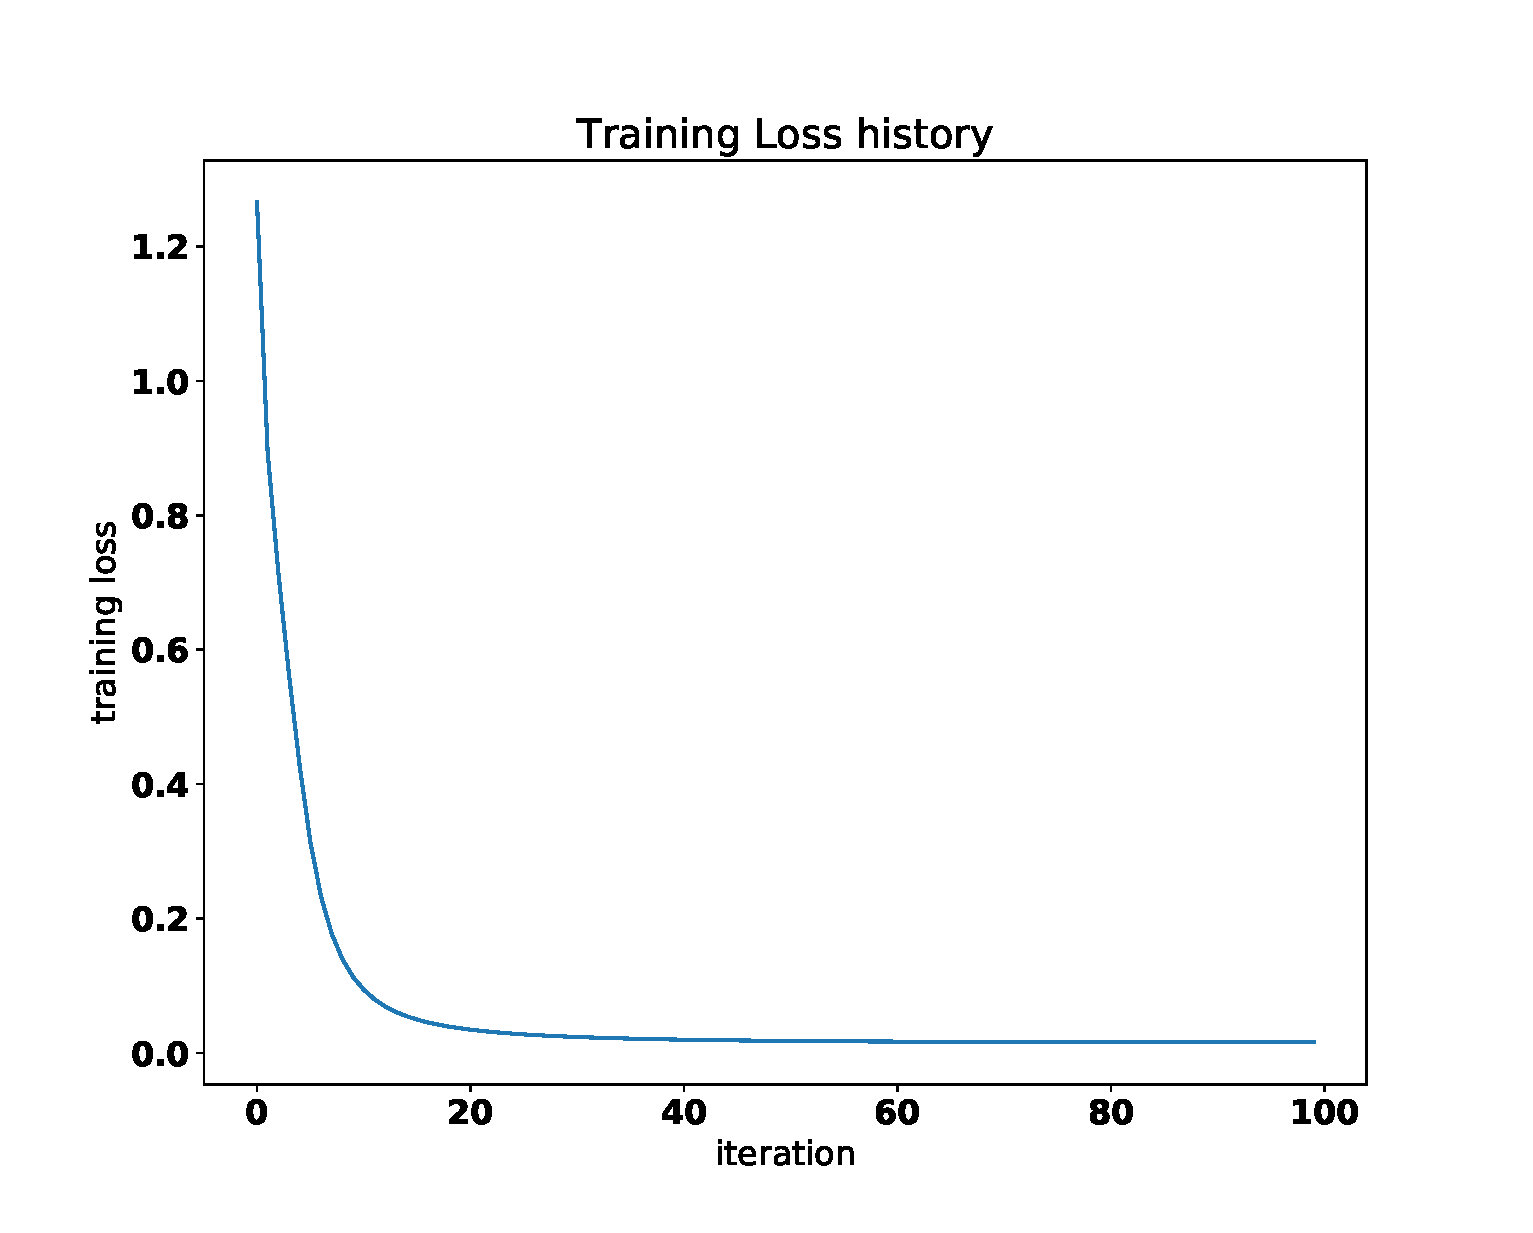
\includegraphics[width=10cm]{a4/toy_lt.eps}
  \end{figure}
  
  针对数据,使用题目中的超参数我们得到约0.29的准确率,作出损失函数和训练、验证准确率随迭代次数变化的规律如图\ref{fig:2}所示。

  \begin{figure}[!ht]
  \centering
  \caption{}\label{fig:2}
  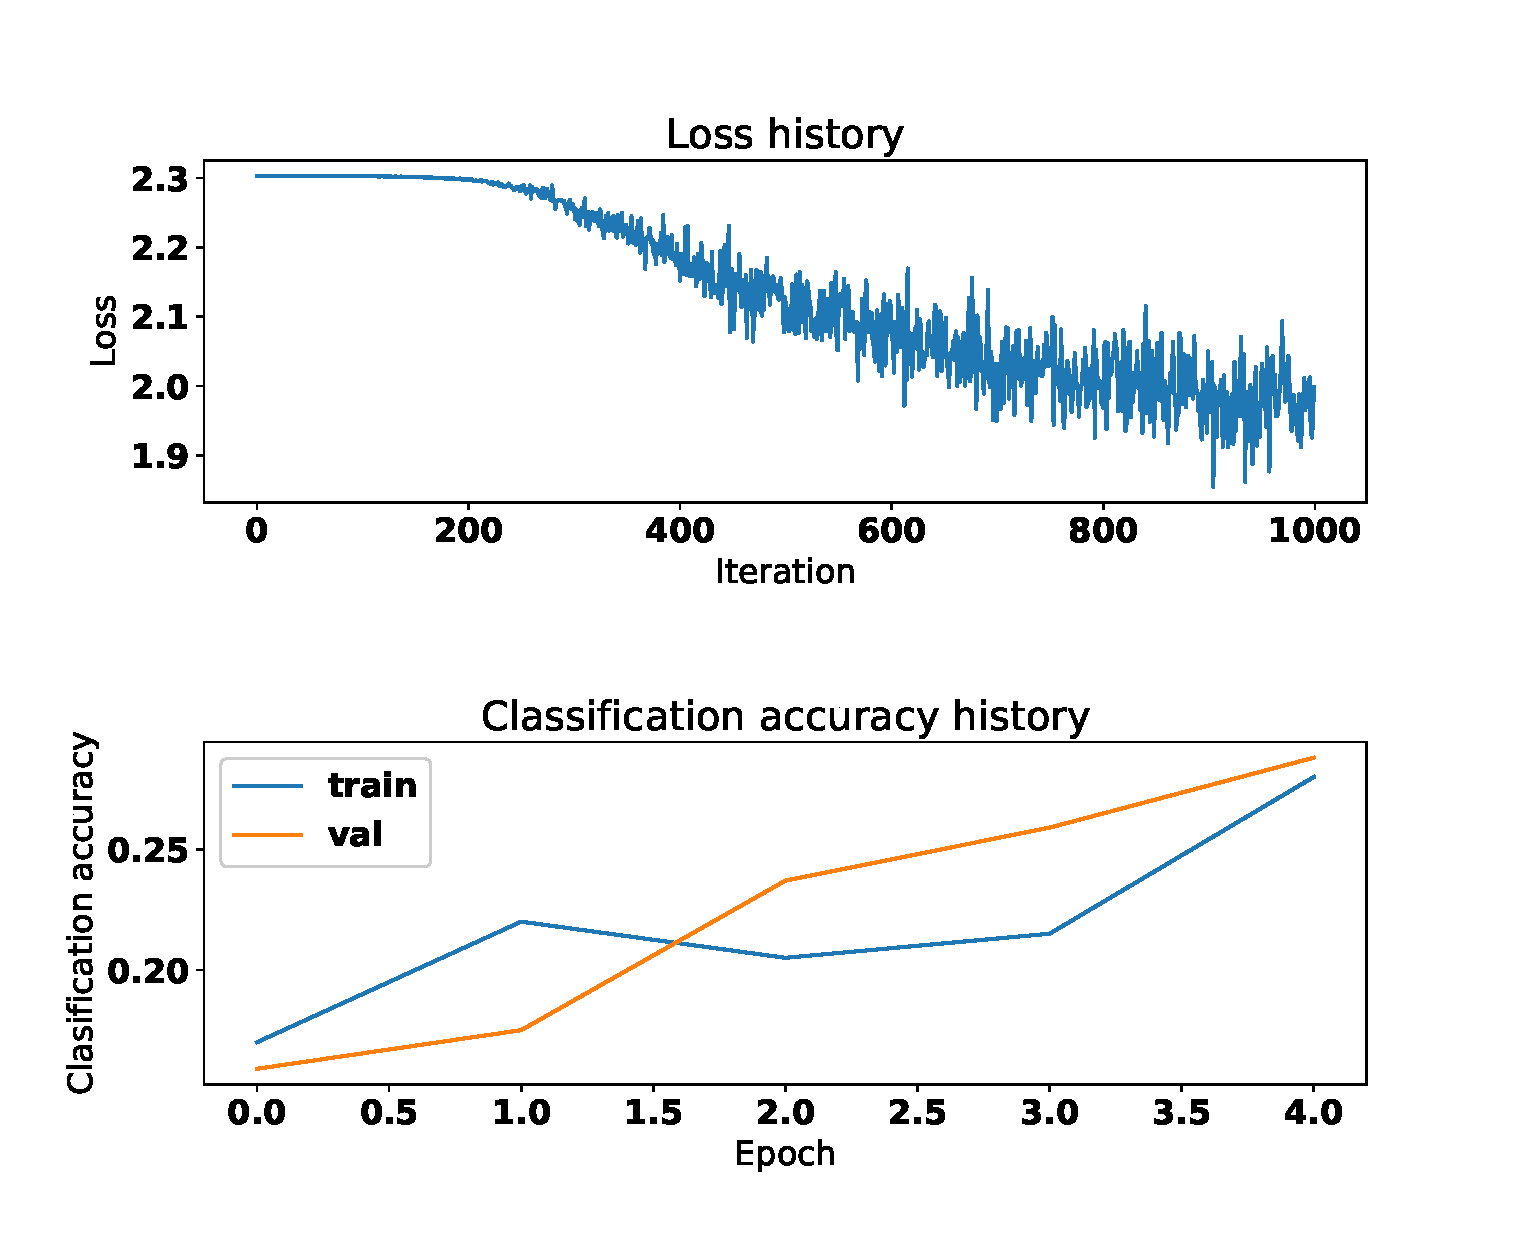
\includegraphics[width=10cm]{a4/default_029acc.eps}
  \end{figure}

  
  对于两层全连接的神经网络,我们针对隐层数量,learning\_rate, 正则化系数,迭代次数共四个超参数进行优化,
  我们采用对四个参数进行离散,在离散后的四维空间进行网格搜索的方法,
  最终优化得到最佳的参数如表\ref{tab}所示。

  \begin{table}[!ht]
  \centering
  \caption{}\label{tab}
  \begin{tabular}{|c|c|}
  \hline
  隐层数量  & 70 \\
  \hline
  learning\_rate & 0.0025\\
  \hline
  正则化系数 & 0.9\\
  \hline
  迭代次数 & 2000\\
  \hline
  Validation accuracy &  0.491\\
  \hline
  Test accuracy &  0.488\\
  \hline
  \end{tabular}
  \end{table}
  
  对于我们找到的最优参数, 网络第一层权系数可视化的结果如图\ref{fig:3}所示。

  \begin{figure}[!ht]
  \centering
  \caption{}\label{fig:3}
  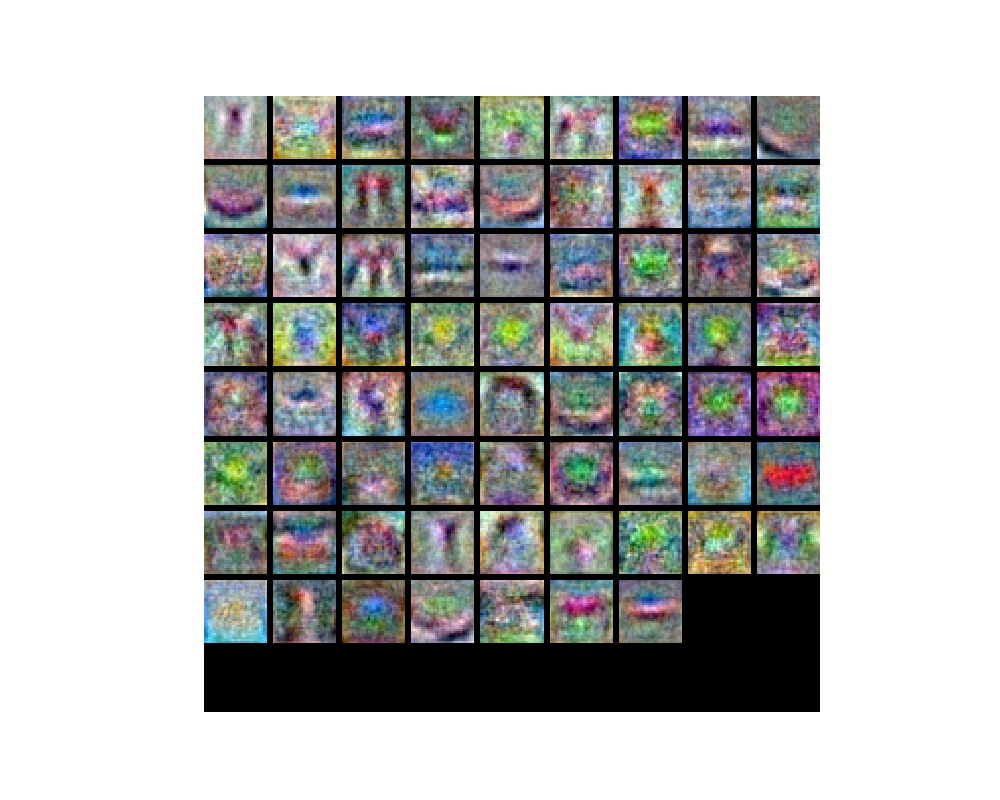
\includegraphics[width=10cm]{a4/net_weights.jpg}
  \end{figure}
  
  寻找最佳参数的python代码如hyperparameter\_tuning.py所示。
  
  \lstinputlisting[language=Python]{a4/hyperparameter_tuning.py}
  
  补全指定函数后的neutral\_net.py文件如下。
  
  \lstinputlisting[language=Python]{a4/cs231n/classifiers/neural_net.py}

  \end{enumerate}

\end{document}
        \begin{equation}
        \end{equation}
%%% Local Variables:
%%% mode: latex
%%% TeX-master: t
%%% End:
 